\chapter{Prenotazioni}
Per effettuare una prenotazione, cliccare la voce ``Calendario'' nel menù in alto alla pagina web.
Selezionare il calendario di propria competenza
\begin{figure}[H]
\centering{}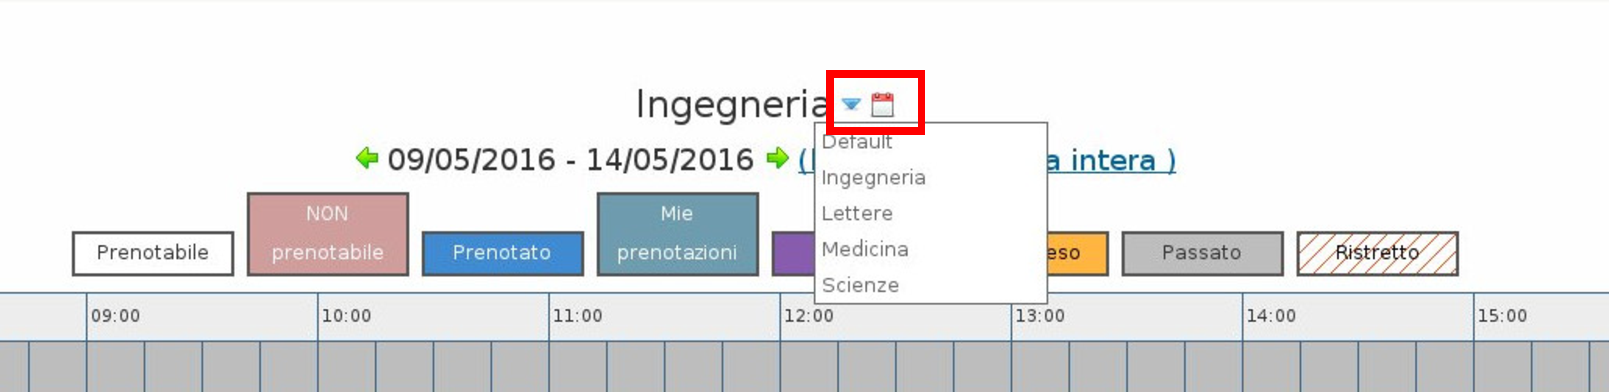
\includegraphics[scale=0.5]{Immagini/calendari_selezione.pdf}
\normalsize
\caption{}
\label{fig:calendari_selezione.pdf}
\end{figure}

e scorrere la pagina fino a trovare la data adatta alla prenotazione. Sulle righe
si avranno tutte le risorse aule disponibili. È possibile modificare i dettagli orari nella schermata
successiva.

Per fare una prenotazione su più giorni della settimana, andare nella zona ``Ripeti'' come in Figura
\ref{fig:prenotazione_ripetizione_1.pdf}

\begin{figure}[H]
\centering{}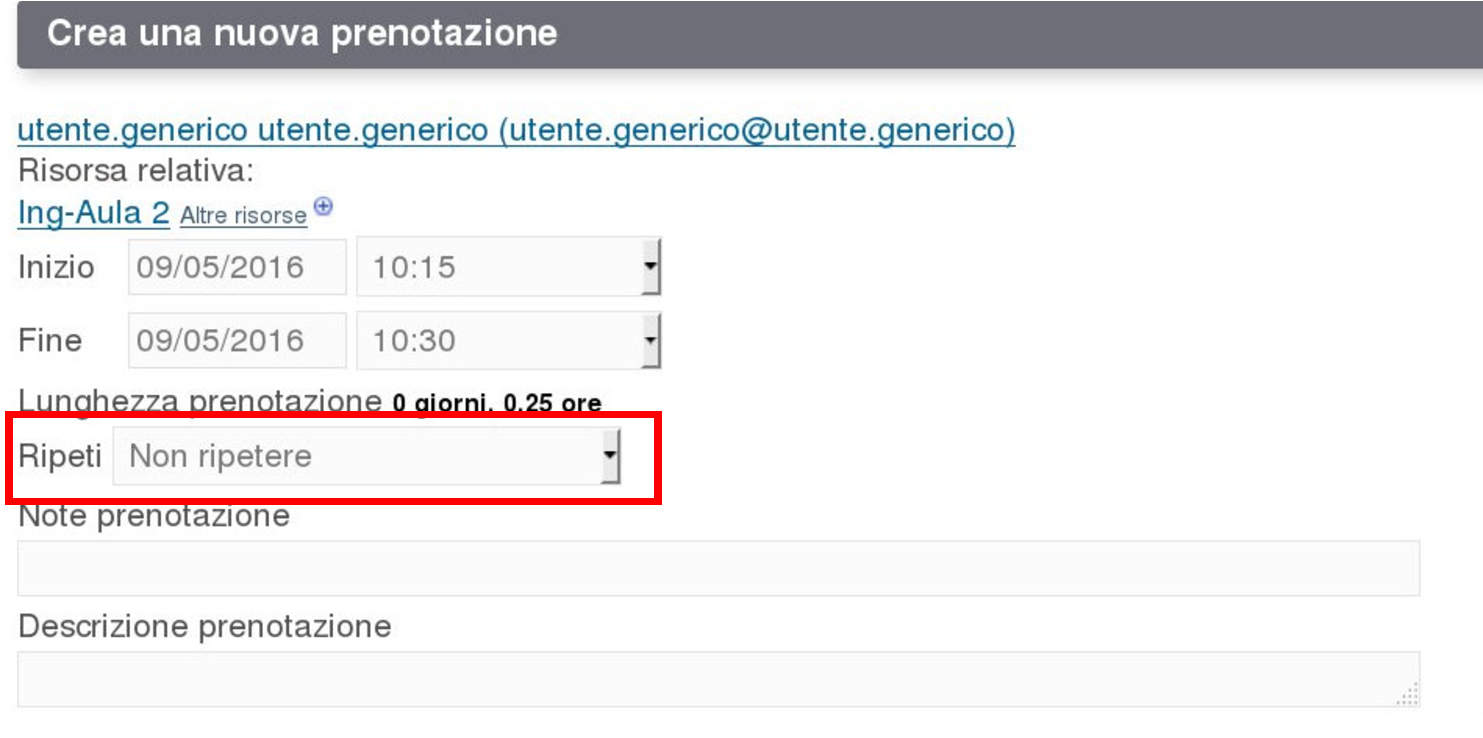
\includegraphics[scale=0.5]{Immagini/prenotazione_ripetizione_1.pdf}
\normalsize
\caption{}
\label{fig:prenotazione_ripetizione_1.pdf}
\end{figure}

e cliccare su ``Settimanale''

\begin{figure}[H]
\centering{}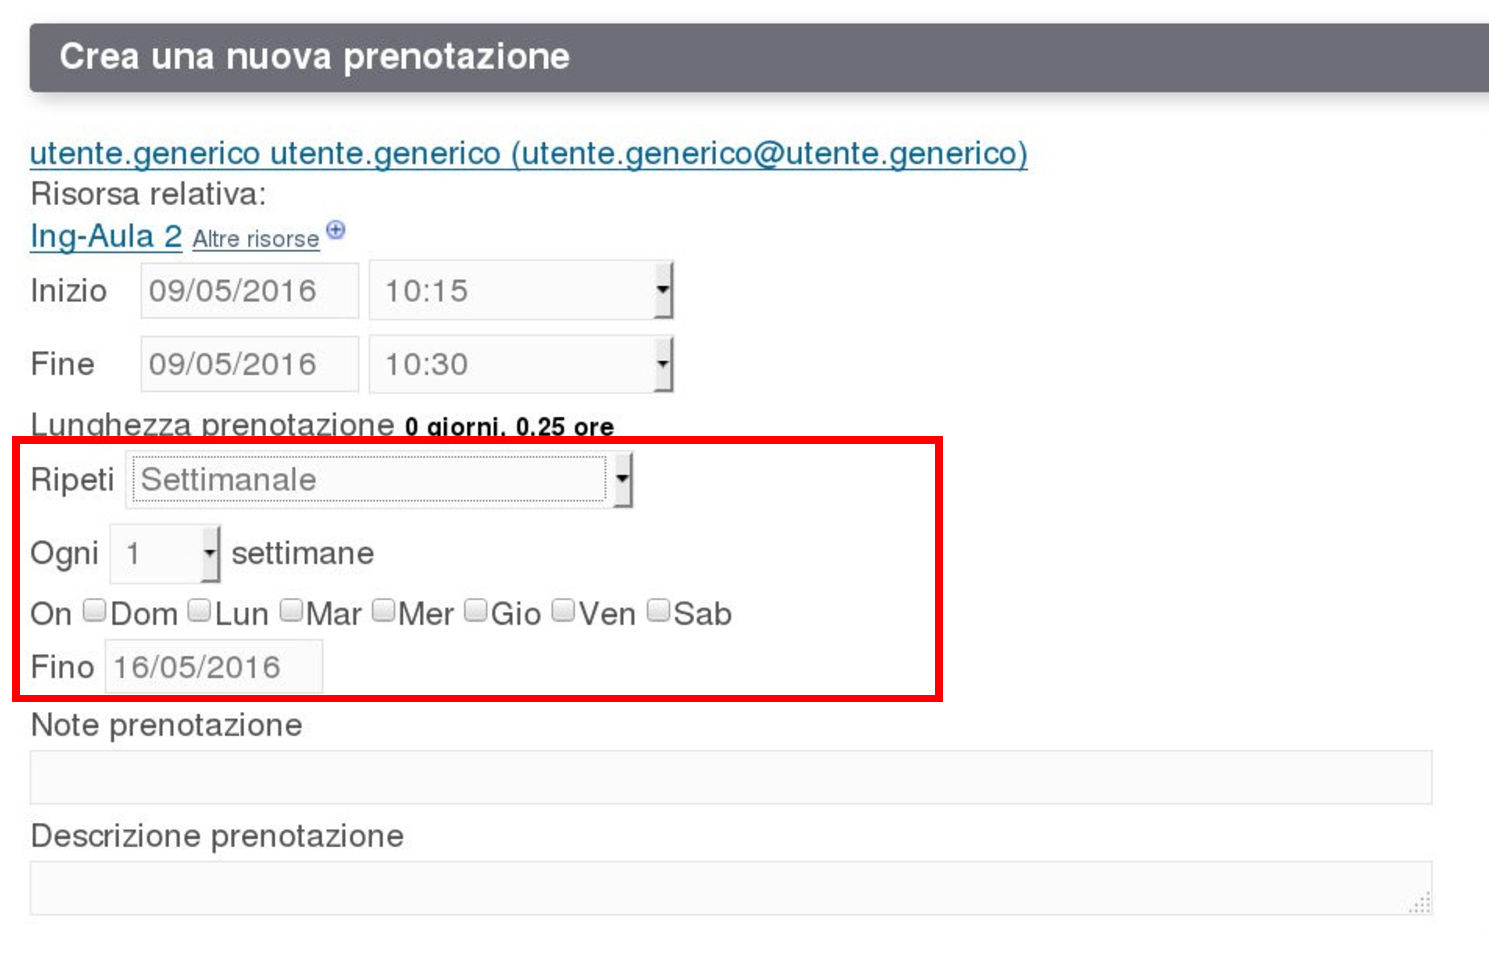
\includegraphics[scale=0.5]{Immagini/prenotazione_ripetizione_2.pdf}
\normalsize
\caption{}
\label{fig:prenotazione_ripetizione_2.pdf}
\end{figure}


Non dimenticare di aggiungere il corso di studi della materia e l'anno corrispondente.


\begin{figure}[H]
\centering{}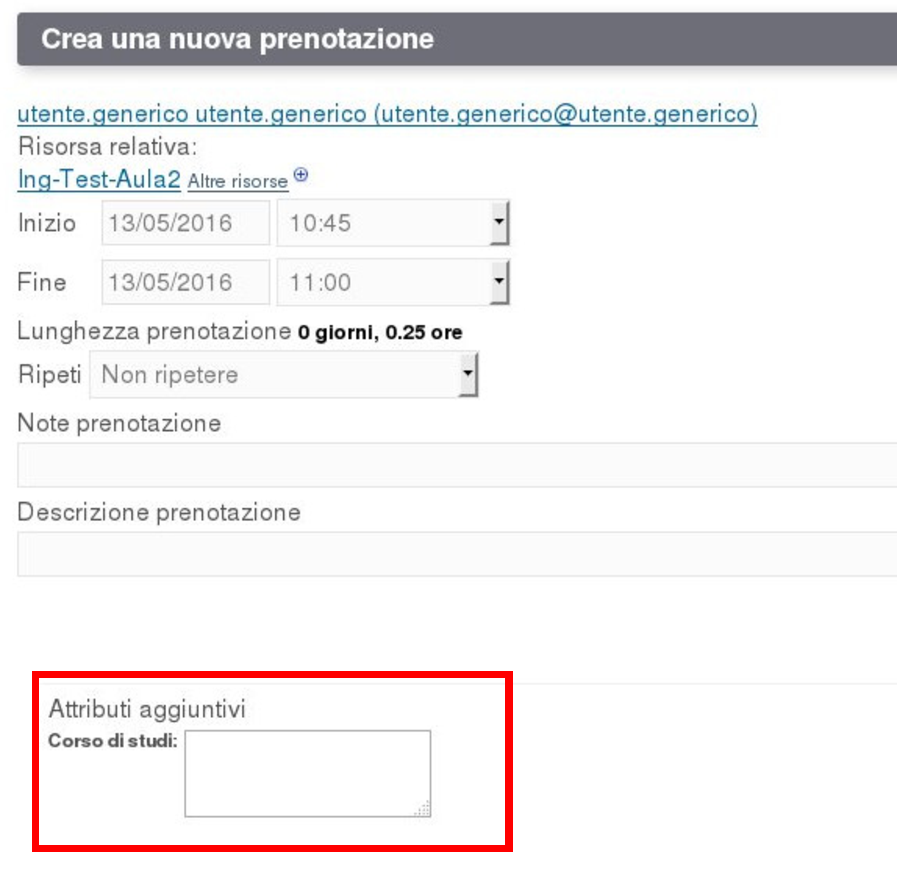
\includegraphics[scale=0.5]{Immagini/prenotazione_attributi.pdf}
\normalsize
\caption{}
\label{fig:prenotazione_attributi.pdf}
\end{figure}

Un esempio può essere

\begin{figure}[H]
 \centering{} Ingegneria informatica II anno
\normalsize
\end{figure}

Nel caso la prenotazione riguardi più corsi di studi, metterne uno per riga